% !TEX root = ../main.tex
% --+ 11.21 SUMMARY +-----------------------------------------------------------
\begin{frame}{Cuts}
    \label{11.21::summary}

    To improve particle quality, three types of cuts are applied:

    \vspace{12pt}

    \begin{itemize}
        \item
            \ef{Tracking cut} to exclude particles that fail a \ef{$\chi^2$ test}: $\chi^2/\text{NDF} < 15$.

        \vspace{6pt}
        \item
            \ef{Geometry cuts} that define a valid analysis region:
            \begin{itemize}
                \vspace{6pt}
                \item
                    Particle vertex is constrained to the beamline: \ef{$\sqrt{v_z^2 + v_y^2} < 4 \text{ cm}$}.

                \vspace{3pt}
                \item
                    Particle vertex originates from the RG-F target: \ef{$-40 \text{ cm} < v_z < z_0 \text{ cm}$}, where \ef{$z_0$} is the $z$ position of the first FMT layer.

                \vspace{3pt}
                \item
                    No fiducial cuts were applied in this study\appref{20.06::fiducial_cuts}.
            \end{itemize}

        \vspace{6pt}
        \item
            \ef{DIS cuts} to narrow down analysis region on DIS.
    \end{itemize}
\end{frame}

% --+ 11.22 DIS CUTS +----------------------------------------------------------
\begin{frame}{DIS Cuts}
    \label{11.22::dis_cuts}

    Three DIS cuts are applied to the trigger $e^-$ of an event to restrict the phase space:

    \begin{itemize}
        \item
            DIS processes require a high enough virtual photon mass: \textcolor{efd_green}{$Q^2 > 1 \text{ GeV}^2$}.

        \item
            To exclude nucleon resonances, the squared mass of the final hadronic state $W^2$\appref{12.14::dis_variables} is restricted: \textcolor{efd_green}{$W^2 > 4 \text{ GeV}^2$}.

        \item
            To mitigate radiative effects, we constrain the Bjorken-Y $Y_b$\appref{12.14::dis_variables}: \textcolor{efd_green}{$Y_b = \nu/E_b < 0.85$}.
    \end{itemize}

    \vspace{-18pt}

    \begin{columns}[onlytextwidth,T]

    \begin{column}{.05\linewidth}\end{column} % Centering column.

    \begin{column}{.44\linewidth}
        \begin{center}
            \begin{figure}[t]
                \centering{
                    \fbox{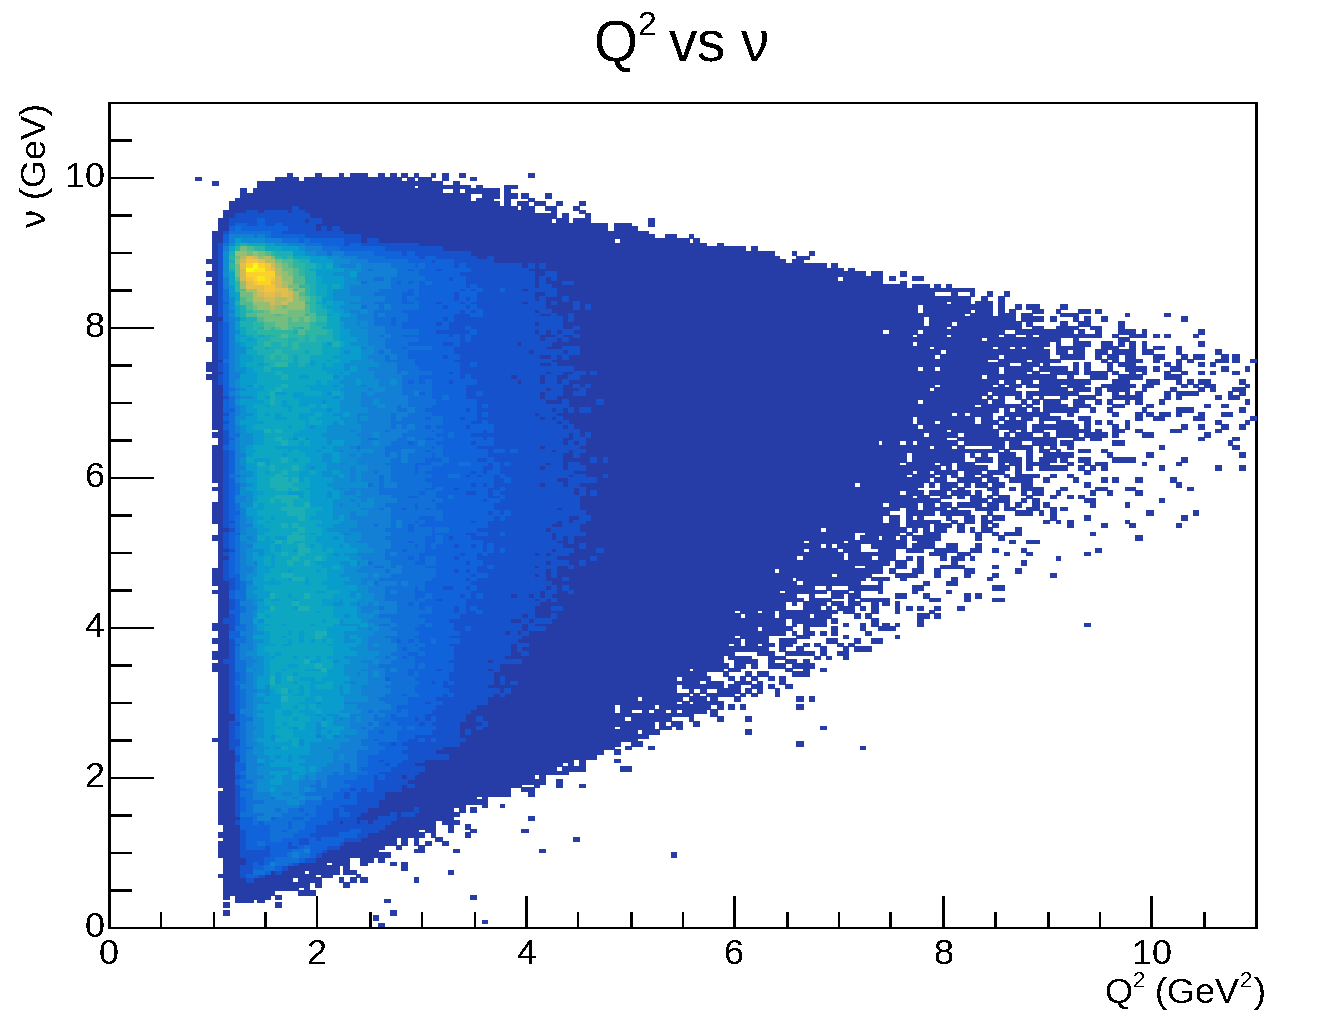
\includegraphics[width=\textwidth]{22nocut.pdf}}
                }
                \scriptsize{\textit{$Q^2$ vs. $\nu$, \ef{no DIS cuts}.}}
            \end{figure}
        \end{center}
    \end{column}

    \begin{column}{.015\linewidth}\end{column} % Centering column.

    \begin{column}{.44\linewidth}
        \begin{center}
            \begin{figure}[t]
                \centering{
                    \fbox{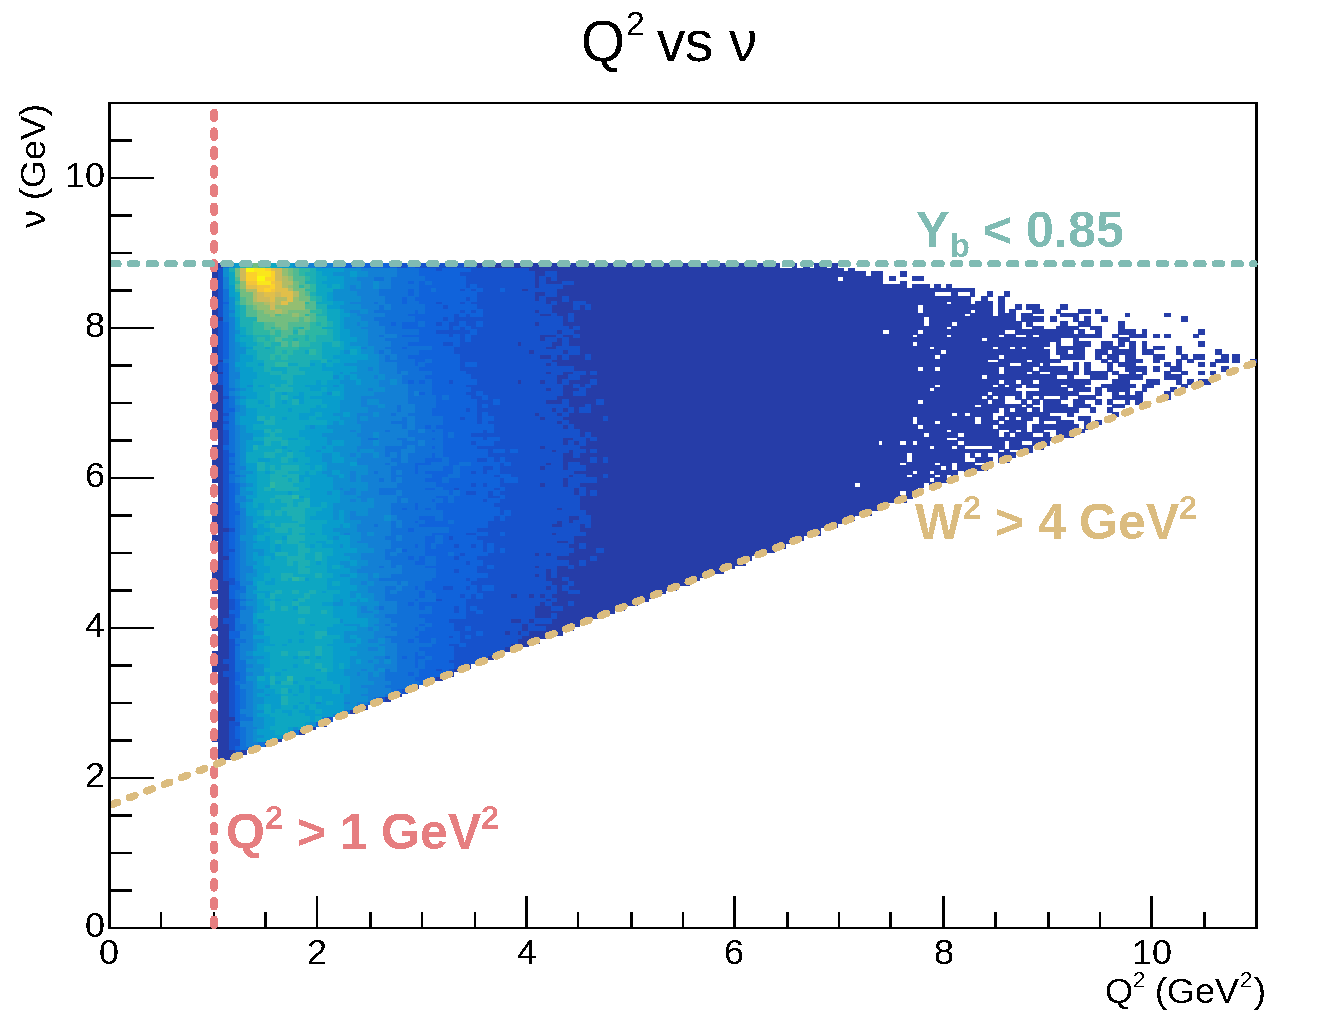
\includegraphics[width=\textwidth]{22wcuts.pdf}}
                }
                \scriptsize{\textit{$Q^2$ vs. $\nu$ \ef{w/ DIS cuts}.}}
            \end{figure}
        \end{center}
    \end{column}

    \begin{column}{.05\linewidth}\end{column} % Centering column.

    \end{columns}
\end{frame}
